% !TeX root = ../thesis.tex

\chapter{引言}
   传统的多线程模型是用共享内存的方式进行同步的。
   但当并行度变高,不确定性就会增加,需要用锁等机制保证正确性。
   由于锁是原子性操作,容易成为性能瓶颈,并且在多线程编程过程中容易出错,产生死锁。
   于是一些进程模型使用消息传递来代替共享内存和锁,认为用通信实现进程同步会更优雅。
   比如在Effective Go中对并发的描述中有这样一句话:
   \textit{“Do not communicate by sharing memory; instead, share memory by communicating."}\cite{1}


   \section{并发进程模型}
   20世纪80年代,英国学者Milner提出了通信系统演算(A Calculus of Communicating System,简称\textbf{CCS})\cite{2},
   同时期Hoare提出了CSP\cite{3},
   Bergstra和Klop等提出了ACP\cite{4},Hennessy提出ATP\cite{5}等使用代数方法研究通信并发系统,统称为进程代数理论。这些代数理论都使用通信而不是共享内存作为进程之间交互的手段。
   前面提到的Golang语言就包含了上述并发通信模型中的CSP模型。

   \subsection{通信系统演算(CCS)}
   Milner的通信系统演算(以下称为CCS)可以表达操作带来的状态迁移,进程的并行执行,多种操作的选择和通道的范围限制。
   这一并发进程模型可以用标记变迁系统(Labled Transition System)表示:

   CCS的语法如下:
   $$S,T:=X\mid \sum_{i\in I}\alpha_i.T_i\mid S\mid T \mid (a)T \mid \mu X.T$$

   其中$S,T$为CCS的代理(agent),$X$为代理变量(agent variables)。索引集合$I$是有限自然数集。
   $Chan$为名字(name)的集合,其中的元素以小写字母表示,
   集合$\overline{Chan}=\{\overline{a}\mid a\in Chan\}$,
   动作集合$Act=Chan\cup \overline{Chan}\cup \{\tau\} $,
   其中的元素用小写希腊字母表示,$\alpha_i\in Act$,$\tau$表示一切内部动作。
   $\sum_{i\in I}\alpha_i.T$为非确定性选择项,若$I=\emptyset$,我们可以将这一项写作$0$。
   $S\mid T$表示$S,T$可以并发执行。$(a)T$为限制(Restriction)或本地化(Localization)操作子,对外隐藏$T$中的$a$通道,
   也可以写为$T\backslash \{a\}$或$T\backslash a$。$\mu X$表示递归(Recursion)操作。
   若一个CCS代理$P$中不含自由变量,称$P$为进程(process)。

   CCS的迁移语义如图~\ref{fig_ccs},表示状态之间的变迁规则,其中$\lambda \in Act$。

   \begin{figure}[!htbp]
    \small
    \centering
    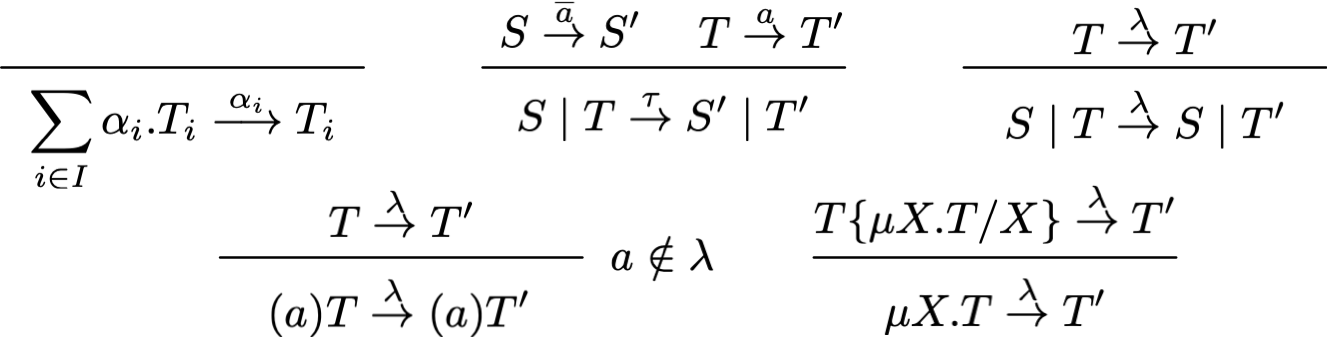
\includegraphics[width=11cm]{../figure/ccs.png}
    \caption[]{CCS迁移语义}
     \label{fig_ccs}
 \end{figure}

   CCS及其扩展模型可以用于并发系统的建模。
   提出CCS时,Milner在\cite{2}中对有界缓冲区,存在并行工作的工人的工厂,支持并行计算的编程语言进行了建模。
   基于CCS的建模还有Guo等的欧洲列车控制系统\cite{16},
   Issad等的铁路系统\cite{17},
   Cleaveland等的图坐标系语言\cite{18}等。
   CCS也可以用来评估系统特性,如判断是否出现死锁。[wiki有一个引用]
   \section{随机进程模型}

   进程代数将进程看作带标号的变迁系统,将并发性归结为非确定性,
   将并发执行的进程看作单个进程所有可能的行为的交错,即交错语义。
   在进程模型中,进程的一个行为通常不是真的随机行为(其实是非确定行为),
   但可能近似的满足某种随机分布。
   而计算机算法都是确定性算法,引入随机性后可以对模型更好的模拟实现。

   作为经典并发模型的扩展,概率进程模型被广为研究。
   其中有对CCS的概率性扩展\cite{9,10},
   概率CSP\cite{11} 和概率ACP\cite{12}等。

   \subsection{A Uniform Approach to Random Process Model}
   Fu提供了一个模型无关的方法—— An Uniform Approach to Random Process Model(后文称为Uniform Approach),
   进程模型扩展为随机进程模型(Random Process Model)。
   Uniform Approach区分了非确定行为和概率性的行为,
   在CCS的基础上建立了Randomized CCS(后文称为RCCS)的语法和等价关系。

   RCCS在CCS的基础上增加了概率选择操作子$\bigoplus_{i\in I}p_i\tau.T_i$,
   其中$0<p_i<1 \wedge \sum_{i\in I}p_i = 1$。
   例如,$S=\frac{1}{3}\tau.T_1+\frac{2}{3}\tau.T_2$意味着$S$经过内部动作到达$T_1$的概率为$\frac{1}{3}$,
   到达$T_2$的概率为$\frac{2}{3}$。

   对应随机选择操作子的迁移语义为:
   \begin{figure}[!htbp]
    \small
    \centering
    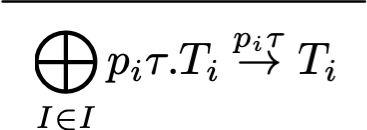
\includegraphics[width=3cm]{../figure/rccs.png}
    \caption[]{}
     \label{fig_rccs}
 \end{figure}

   由于Uniform Approach具有模型无关性,我们可以用它来扩展其他的进程模型,
   进而使非概率模型概率化。概率化后,模型将会拥有更可计算、可模拟的性质。
   进而可以更好的对现实问题进行仿真和分析。

\section{本章小结}
本章引入了通信并发系统的概念,
介绍了一种通信并发演算CCS的语法、迁移语义以及适用的应用场景。
出于随机性在计算机科学中的重要性的考虑,
我们引入了一种对进程模型进行概率化扩展的方法The Uniform Approach to Random Process Model,
简单地介绍了Uniform Approach如何对CCS进行概率扩展,
并分析了概率化扩展通信并发模型的意义。